%%%%%%%%%%%%%%%%%%%%%%%%%%%%%%%%%%%%%%%%%
% Beamer Presentation
% LaTeX Template
% Version 1.0 (10/11/12)
%
% This template has been downloaded from:
% http://www.LaTeXTemplates.com
%
% License:
% CC BY-NC-SA 3.0 (http://creativecommons.org/licenses/by-nc-sa/3.0/)
%
%%%%%%%%%%%%%%%%%%%%%%%%%%%%%%%%%%%%%%%%%

%----------------------------------------------------------------------------------------
%	PACKAGES AND THEMES
%----------------------------------------------------------------------------------------

\documentclass{beamer}

\mode<presentation> {
\usetheme{Singapore}
\usecolortheme{rose}
\setbeamertemplate{footline}[page number]

\setbeamertemplate{navigation symbols}{}
}

\usepackage{graphicx} % Allows including images
\usepackage{booktabs} % Allows the use of \toprule, \midrule and \bottomrule in tables
\usepackage{listings}
\usepackage{xcolor}
\usepackage{color}

\colorlet{punct}{red!60!black}
\definecolor{background}{HTML}{EEEEEE}
\definecolor{delim}{RGB}{25,134,57}
\colorlet{numb}{magenta!60!black}

\lstdefinelanguage{json}{
    basicstyle=\normalfont\ttfamily,
    numbers=left,
    numberstyle=\scriptsize,
    stepnumber=1,
    numbersep=8pt,
    showstringspaces=false,
    breaklines=true,
    frame=lines,
    backgroundcolor=\color{background},
    literate=
     *{0}{{{\color{numb}0}}}{1}
      {1}{{{\color{numb}1}}}{1}
      {2}{{{\color{numb}2}}}{1}
      {3}{{{\color{numb}3}}}{1}
      {4}{{{\color{numb}4}}}{1}
      {5}{{{\color{numb}5}}}{1}
      {6}{{{\color{numb}6}}}{1}
      {7}{{{\color{numb}7}}}{1}
      {8}{{{\color{numb}8}}}{1}
      {9}{{{\color{numb}9}}}{1}
      {:}{{{\color{punct}{:}}}}{1}
      {,}{{{\color{punct}{,}}}}{1}
      {\{}{{{\color{delim}{\{}}}}{1}
      {\}}{{{\color{delim}{\}}}}}{1}
      {[}{{{\color{delim}{[}}}}{1}
      {]}{{{\color{delim}{]}}}}{1},
}
%----------------------------------------------------------------------------------------
%	TITLE PAGE
%----------------------------------------------------------------------------------------

\title[AureliaJS]{AureliaJS}
\author{Jesse Javier Cogollo Alvarez}
\institute[EAFIT - TalosDigital]
{
Developer by passion \\
\medskip
\textit{email: cogollo87@gmail.com} \\~\\
\textit{MedellinJS}
}
%\date{\today} % Date, can be changed to a custom date
\begin{document}

\begin{frame}
\titlepage % Print the title page as the first slide
\end{frame}

\begin{frame}
\frametitle{Contenido} % Table of contents slide, comment this block out to remove it
\tableofcontents % Throughout your presentation, if you choose to use \section{} and \subsection{} commands, these will automatically be printed on this slide as an overview of your presentation
\end{frame}

%----------------------------------------------------------------------------------------
%	PRESENTATION SLIDES
%----------------------------------------------------------------------------------------

%------------------------------------------------
\section{AureliaJS} % Sections can be created in order to organize your presentation into discrete blocks, all sections and subsections are automatically printed in the table of contents as an overview of the talk
%------------------------------------------------
\begin{frame}
\frametitle{Que es Aurelia?}
Aurelia is a next generation JavaScript client framework that leverages simple conventions to empower your creativity.
{\color{blue}\url{http://aurelia.io/}}
\\~\\
Rob Eisenberg

{\color{blue}\url{robeisenberg.com}}

%\begin{figure}
%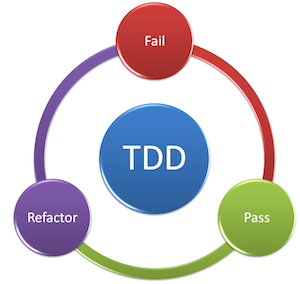
\includegraphics[width=0.3\linewidth]{tdd.png}
%\end{figure}
\end{frame}

%------------------------------------------------
\begin{frame}
\frametitle{Caracteristicas}
\begin{columns}[c] % The "c" option specifies centered vertical alignment while the "t" option is used for top vertical alignment

\column{.45\textwidth} % Left column and width
\begin{enumerate}
\item \textbf{Forward-thinking}
\item[•]
\item[•]
\item[•]
\item[•]
\item[•]
\item[•]
\item[•]
\end{enumerate}

\column{.5\textwidth} % Right column and width
Escrito con ES6 y ES7. se integra con web components. no tiene dependencias externas (excepto polyfills).
\end{columns}
\end{frame}

%------------------------------------------------

\begin{frame}
\frametitle{Caracteristicas}
\begin{columns}[c] % The "c" option specifies centered vertical alignment while the "t" option is used for top vertical alignment

\column{.45\textwidth} % Left column and width
\begin{enumerate}
\item \textbf{Forward-thinking}
\item \textbf{Modern Architecture}
\item[•]
\item[•]
\item[•]
\item[•]
\item[•]
\item[•]
\end{enumerate}

\column{.5\textwidth} % Right column and width
Aurelia esta compuesto por pequenos modulos. Utiliados juntos como un completo framework. Pero tambien permite personalizarlo con diferentes modulos.
\end{columns}
\end{frame}

%------------------------------------------------
\begin{frame}
\frametitle{Caracteristicas}
\begin{columns}[c] % The "c" option specifies centered vertical alignment while the "t" option is used for top vertical alignment

\column{.45\textwidth} % Left column and width
\begin{enumerate}
\item \textbf{Forward-thinking}
\item \textbf{Modern Architecture}
\item \textbf{Two-Way Databinding}
\item[•]
\item[•]
\item[•]
\item[•]
\item[•]
\end{enumerate}

\column{.5\textwidth} % Right column and width
Aurelia tiene una poderosa two-way binding. el cual utiliza tecnicas adaptativas para utilizar el mecanismo mas eficiente para observar cada propiedad. Object.observer
\end{columns}
\end{frame}

%------------------------------------------------
\begin{frame}
\frametitle{Caracteristicas}
\begin{columns}[c] % The "c" option specifies centered vertical alignment while the "t" option is used for top vertical alignment

\column{.45\textwidth} % Left column and width
\begin{enumerate}
\item \textbf{Forward-thinking}
\item \textbf{Modern Architecture}
\item \textbf{Two-Way Databinding}
\item \textbf{Extensible HTML}
\item[•]
\item[•]
\item[•]
\item[•]
\end{enumerate}

\column{.5\textwidth} % Right column and width
La extensibilidad HTML de Aurelia permite crear elementos HTML personalizados, anadir nuevos comportamientos para elementos ya existentes.
\end{columns}
\end{frame}

%------------------------------------------------
\begin{frame}
\frametitle{Caracteristicas}
\begin{columns}[c] % The "c" option specifies centered vertical alignment while the "t" option is used for top vertical alignment

\column{.45\textwidth} % Left column and width
\begin{enumerate}
\item \textbf{Forward-thinking}
\item \textbf{Modern Architecture}
\item \textbf{Two-Way Databinding}
\item \textbf{Extensible HTML}
\item \textbf{Routing and UI Composition}
\item[•]
\item[•]
\item[•]
\end{enumerate}

\column{.5\textwidth} % Right column and width
Router con acoplamiento activo, patrones de ruta dinamica, activacion de pantallas asincronicamente, etc.
\end{columns}
\end{frame}

%------------------------------------------------
\begin{frame}
\frametitle{Caracteristicas}
\begin{columns}[c] % The "c" option specifies centered vertical alignment while the "t" option is used for top vertical alignment

\column{.45\textwidth} % Left column and width
\begin{enumerate}
\item \textbf{Forward-thinking}
\item \textbf{Modern Architecture}
\item \textbf{Two-Way Databinding}
\item \textbf{Extensible HTML}
\item \textbf{Routing and UI Composition}
\item \textbf{MV* with Conventions}
\item[•]
\item[•]
\end{enumerate}

\column{.5\textwidth} % Right column and width
Quieres invertir tiempo en escribir codigo de configuracion? Aurelia maneja una convecion simple.
\end{columns}
\end{frame}

%------------------------------------------------

%------------------------------------------------
\begin{frame}
\frametitle{Caracteristicas}
\begin{columns}[c] % The "c" option specifies centered vertical alignment while the "t" option is used for top vertical alignment

\column{.45\textwidth} % Left column and width
\begin{enumerate}
\item \textbf{Forward-thinking}
\item \textbf{Modern Architecture}
\item \textbf{Two-Way Databinding}
\item \textbf{Extensible HTML}
\item \textbf{Routing and UI Composition}
\item \textbf{MV* with Conventions}
\item \textbf{Broad Language Support}
\item[•]
\end{enumerate}

\column{.5\textwidth} % Right column and width
Utiliza ES5, ES6, TypeScript, AtScript, CoffeeScript.
\end{columns}
\end{frame}

%------------------------------------------------

%------------------------------------------------
\begin{frame}
\frametitle{Caracteristicas}
\begin{columns}[c] % The "c" option specifies centered vertical alignment while the "t" option is used for top vertical alignment

\column{.45\textwidth} % Left column and width
\begin{enumerate}
\item \textbf{Forward-thinking}
\item \textbf{Modern Architecture}
\item \textbf{Two-Way Databinding}
\item \textbf{Extensible HTML}
\item \textbf{Routing and UI Composition}
\item \textbf{MV* with Conventions}
\item \textbf{Broad Language Support}
\item \textbf{Testable}
\end{enumerate}

\column{.5\textwidth} % Right column and width
combinando modulos ES6 con contenedor inyeccion de dependencias. se hace mas facil crear codigo altamente cohesivo y bajo acoplamiento. haciendo las pruebas unitarias algo facil.
\end{columns}
\end{frame}

%------------------------------------------------

\begin{frame}
\frametitle{Como empezar - Estructura}
Descargamos la ultima version del skeleton de aurelia.
\\~\\
{\color{blue}\url{https://github.com/aurelia/skeleton-navigation/releases/tag/0.15.1}}
\\~\\
descomprimimos y ya tenemos una estrutura lista para utilizar:
\begin{itemize}
\item build (configuracion gulp).
\item doc (documentacion).
\item src (codificacion).
\item styles (estilos CSS).
\item test (pruebas).
\item README.md (instrucciones para utilizar AureliaJS).
\end{itemize}
\end{frame}

%------------------------------------------------

%------------------------------------------------

%\begin{frame}
%\frametitle{Como empezar}
%Descargamos la ultima version del skeleton de aurelia.
%\begin{itemize}
%\item No utilizan el modelo relacional.
%\item Corren bien en clusters.
%\item Open-source.
%\item sin esquemas.
%\item El resultado mas importante del aumento de las bases de datos NoSQL es la {\color{green}Persistencia %Poliglota}.
%\end{itemize}
%{\color{blue}\url{Descargar: https://github.com/aurelia/skeleton-navigation/releases/tag/0.15.1}}
%\end{frame}

%------------------------------------------------

%------------------------------------------------
\begin{frame}
\frametitle{Modulos}
\begin{columns}[c] % The "c" option specifies centered vertical alignment while the "t" option is used for top vertical alignment

\column{.45\textwidth} % Left column and width
\begin{itemize}
\item \textbf{logging}
\end{itemize}

\column{.5\textwidth} % Right column and width
Esta libreria es parte de la plataforma aurelia y contiene un "Appender" para el logging.
\\~\\
uso:
welcome.js
\end{columns}
\end{frame}

%------------------------------------------------
\begin{frame}
\frametitle{Modulos}
\begin{columns}[c] % The "c" option specifies centered vertical alignment while the "t" option is used for top vertical alignment

\column{.45\textwidth} % Left column and width
\begin{itemize}
\item \textbf{Plugins}
\end{itemize}

\column{.5\textwidth} % Right column and width
Aurelia permite crear e implementar plugins que se adaptan a Aurelia.
Estos plugins se configuran en:
implementación: index.html
uso: animation-main.js
\end{columns}
\end{frame}

%------------------------------------------------
%\begin{frame}
%\frametitle{Caracteristicas}
%\begin{columns}[c] % The "c" option specifies centered vertical alignment while the "t" option is used for top %vertical alignment

%\column{.45\textwidth} % Left column and width
%\begin{itemize}
%\item \textbf{Aurelia Object}
%\end{itemize}

%\column{.5\textwidth} % Right column and width
%Aurelia Object (TODO)
%\end{columns}
%\end{frame}

%------------------------------------------------
\begin{frame}
\frametitle{Vistas y vistas modelos}
\begin{columns}[c]

\column{.45\textwidth} % Left column and width
\begin{itemize}
\item \textbf{DI inyeccion de dependencias}
\end{itemize}

\column{.5\textwidth} % Right column and width
Los AureliaElements son creados como clases los cuales son instaciados por el framework usando contenedor de inyeccion de dependencias.
\\~\\
uso: flickr.js
\end{columns}
\end{frame}

%------------------------------------------------
%\begin{frame}
%\frametitle{Vistas y vistas modelos}
%\begin{columns}[c] % The "c" option specifies centered vertical alignment while the "t" option is used for top vertical alignment

%\column{.45\textwidth} % Left column and width
%\begin{itemize}
%\item \textbf{Modelos de vista padre}
%\end{itemize}

%\column{.5\textwidth} % Right column and width
%Modelos de vista padre (TODO)
%\end{columns}
%\end{frame}

%------------------------------------------------
\begin{frame}
\frametitle{Vistas y vistas modelos}
\begin{columns}[c] % The "c" option specifies centered vertical alignment while the "t" option is used for top vertical alignment

\column{.45\textwidth} % Left column and width
\begin{itemize}
\item \textbf{Plantillas}
\end{itemize}

\column{.5\textwidth} % Right column and width
El motor de plantillas de aurelia es el encargado de cargar las vistas y sus recursos, compilando su HTML para un optimo desempeno y renderizando el UI en la pantalla.
\\~\\
<template> </template>. Todo lo que este adentro de esas etiquetas sera administrado por aurelia.
\\~\\
uso: welcome.html
\end{columns}
\end{frame}

\section{DEMO}
%------------------------------------------------
\begin{frame}
\frametitle{Databiding}
\begin{columns}[c]

\column{.45\textwidth} % Left column and width
\begin{itemize}
\item \textbf{Que es}
\end{itemize}

\column{.5\textwidth} % Right column and width
El Databinding nos permite enlazar el estado y comportamiento en un objeto(js) y una vista(html).
\\~\\
Cualquier cambio es enlazado y/o sincronizado en una o varias direcciones. Se puede diferenciar en la vista por que el elemento va seguido de un punto en el atributo con el valor (bind, one-way, two-way o one-time).
\\~\\
implementación: welcome.html
\end{columns}
\end{frame}
%------------------------------------------------
\begin{frame}
\frametitle{Bindings}
\begin{columns}[c]

\column{.45\textwidth} % Left column and width
\begin{itemize}
\item \textbf{delegate, trigger and call}
\end{itemize}

\column{.5\textwidth} % Right column and width
Los bindings no solamente conectan elementos o atributos. Tambien son utilizados para lanzar comportamientos.
Se recomienda utilizar el delegate por defecto por que es el mas eficiente al utilizar la memoria y la cpu.
\\~\\
Implementation: TODO
\end{columns}
\end{frame}
%------------------------------------------------
\begin{frame}
\frametitle{Bindings}
\begin{columns}[c]

\column{.45\textwidth} % Left column and width
\begin{itemize}
\item \textbf{string interpolation}
\end{itemize}

\column{.5\textwidth} % Right column and width
Sintaxis: \${nameVariable}. es un binding de un solo camino, la cual la salida se convierte en un string.
\\~\\
Implementacion: welcome.html
\end{columns}
\end{frame}
%------------------------------------------------
\begin{frame}
\frametitle{Bindings}
\begin{columns}[c]

\column{.45\textwidth} % Left column and width
\begin{itemize}
\item \textbf{ref}
\end{itemize}
\column{.5\textwidth} % Right column and width
Es especial para conectar elementos personalizados, utilizando esta tecnica puedes conectar diferentes componentes.
\\~\\
Implementacion: TODO
\end{columns}
\end{frame}
%------------------------------------------------
\begin{frame}
\frametitle{Bindings}
\begin{columns}[c]

\column{.45\textwidth} % Left column and width
\begin{itemize}
\item \textbf{select elements}
\end{itemize}

\column{.5\textwidth} % Right column and width
"value.bind" es un HTMLSelectElement que tiene un comportamiento especial para soportar seleccion simple y seleccion multiple de valores. normalmente se combina con el elemento repeat. Pero existe otro elemento especial que permite trabajar con objetos "model.bind".
\\~\\
Implementacion: TODO
\end{columns}
\end{frame}
%------------------------------------------------
\begin{frame}
\frametitle{Bindings}
\begin{columns}[c]

\column{.45\textwidth} % Left column and width
\begin{itemize}
\item \textbf{radios}
\end{itemize}

\column{.5\textwidth} % Right column and width
"checked.bind" es un HTMLInputElement tiene un comportamiento especial para soportar binding no booleano, como strings y objetos.
\\~\\
Implementacion: TODO
\end{columns}
\end{frame}
%------------------------------------------------
\begin{frame}
\frametitle{Bindings}
\begin{columns}[c]

\column{.45\textwidth} % Left column and width
\begin{itemize}
\item \textbf{checkboxes}
\end{itemize}

\column{.5\textwidth} % Right column and width
\\~\\
Implementacion: TODO
\end{columns}
\end{frame}
%------------------------------------------------
\begin{frame}
\frametitle{Bindings}
\begin{columns}[c]

\column{.45\textwidth} % Left column and width
\begin{itemize}
\item \textbf{InnerHTML}
\end{itemize}

\column{.5\textwidth} % Right column and width
podemos hacer binding de los elementos innerHTMl con el atributo innerhtml.
\\~\\
Implementacion: TODO
\end{columns}
\end{frame}
%------------------------------------------------
\begin{frame}
\frametitle{Bindings}
\begin{columns}[c]
\column{.45\textwidth} % Left column and width
\begin{itemize}
\item \textbf{textContent}
\end{itemize}
\column{.5\textwidth} % Right column and width
Podemos hacer binding de los elementos textContect con el atributo textcontent.
\\~\\
Implementacion: TODO
\end{columns}
\end{frame}
%------------------------------------------------
\begin{frame}
\frametitle{Bindings}
\begin{columns}[c]
\column{.45\textwidth} % Left column and width
\begin{itemize}
\item \textbf{style}
\end{itemize}
\column{.5\textwidth} % Right column and width
Podemos hacer binding a los string css u objetos en un elemento style.
\\~\\
Implementacion: TODO
\end{columns}
\end{frame}
%------------------------------------------------
\begin{frame}
\frametitle{Bindings}
\begin{columns}[c]
\column{.45\textwidth} % Left column and width
\begin{itemize}
\item \textbf{adaptive binding}
\end{itemize}

\column{.5\textwidth} % Right column and width
\\~\\
Implementacion: TODO Important
\end{columns}
\end{frame}
%------------------------------------------------
\begin{frame}
\frametitle{HTML Extensions}
\begin{columns}[c]
\column{.45\textwidth} % Left column and width
\begin{itemize}
\item \textbf{show}
\end{itemize}

\column{.5\textwidth} % Right column and width
\\~\\
Nos permite condicionar si un elemento o elementos seran visibles o no en el DOM
Implementacion: TODO
\end{columns}
\end{frame}
%------------------------------------------------
\begin{frame}
\frametitle{HTML Extensions}
\begin{columns}[c]
\column{.45\textwidth} % Left column and width
\begin{itemize}
\item \textbf{if}
\end{itemize}

\column{.5\textwidth} % Right column and width
Tiene el mismo comportamiento que el "show". lo que lo hace diferente es que esta etiqueta si remueve el componente del DOM.
\\~\\
Implementacion: TODO Important
\end{columns}
\end{frame}
%------------------------------------------------
\begin{frame}
\frametitle{HTML Extensions}
\begin{columns}[c]
\column{.45\textwidth} % Left column and width
\begin{itemize}
\item \textbf{repeat}
\end{itemize}

\column{.5\textwidth} % Right column and width
Este atributo permite renderizar un template multiples veces y trabaja en conjunto con el ".for"
\\~\\
Implementacion: TODO Important
\end{columns}
\end{frame}
%------------------------------------------------
\begin{frame}
\frametitle{HTML Extensions}
\begin{columns}[c]
\column{.45\textwidth} % Left column and width
\begin{itemize}
\item \textbf{repeat \$parent}
\end{itemize}

\column{.5\textwidth} % Right column and width
permite acceder a las propiedades de la viewModel.
\\~\\
Implementacion: TODO Important
\end{columns}
\end{frame}
%------------------------------------------------
\begin{frame}
\frametitle{HTML Extensions}
\begin{columns}[c]
\column{.45\textwidth} % Left column and width
\begin{itemize}
\item \textbf{repeat \$index}
\end{itemize}

\column{.5\textwidth} % Right column and width
Es el index del item en el array
\\~\\
Implementacion: TODO Important
\end{columns}
\end{frame}
%------------------------------------------------
\begin{frame}
\frametitle{HTML Extensions}
\begin{columns}[c]
\column{.45\textwidth} % Left column and width
\begin{itemize}
\item \textbf{repeat \$first}
\end{itemize}

\column{.5\textwidth} % Right column and width
es verdadero si es el primer item del array
\\~\\
Implementacion: TODO Important
\end{columns}
\end{frame}
%------------------------------------------------
\begin{frame}
\frametitle{HTML Extensions}
\begin{columns}[c]
\column{.45\textwidth} % Left column and width
\begin{itemize}
\item \textbf{repeat \$last}
\end{itemize}

\column{.5\textwidth} % Right column and width
es verdadero si es el ultimo item del array.
\\~\\
Implementacion: TODO Important
\end{columns}
\end{frame}
%------------------------------------------------
\begin{frame}
\frametitle{HTML Extensions}
\begin{columns}[c]
\column{.45\textwidth} % Left column and width
\begin{itemize}
\item \textbf{repeat \$even}
\end{itemize}

\column{.5\textwidth} % Right column and width
es verdadero si el item es un numero par
\\~\\
Implementacion: TODO Important
\end{columns}
\end{frame}
%------------------------------------------------
\begin{frame}
\frametitle{HTML Extensions}
\begin{columns}[c]
\column{.45\textwidth} % Left column and width
\begin{itemize}
\item \textbf{repeat \$odd}
\end{itemize}

\column{.5\textwidth} % Right column and width
es verdadero si el item es un numero impar
\\~\\
Implementacion: TODO Important
\end{columns}
\end{frame}
%------------------------------------------------
%\begin{frame}
%\frametitle{HTML Extensions}
%\begin{columns}[c]
%\column{.45\textwidth} % Left column and width
%\begin{itemize}
%\item \textbf{compose}
%\end{itemize}

%\column{.5\textwidth} % Right column and width

%\\~\\
%Implementacion: TODO Important
%\end{columns}
%\end{frame}
%------------------------------------------------
%\begin{frame}
%\frametitle{HTML Extensions}
%\begin{columns}[c]
%\column{.45\textwidth} % Left column and width
%\begin{itemize}
%\item \textbf{\$global behavior}
%\end{itemize}

%\column{.5\textwidth} % Right column and width
%\\~\\
%Implementacion: TODO Important
%\end{columns}
%\end{frame}
%------------------------------------------------
\begin{frame}
\frametitle{Routing}
\begin{columns}[c]
\column{.45\textwidth} % Left column and width
\begin{itemize}
\item \textbf{descripcion}
\end{itemize}

\column{.5\textwidth} % Right column and width
Cuando implementas enrutadores, tienes varias posibilidades de implementarlo, como: navegacion de la App, dashboards y MDI interfaces.
\\~\\
El Routing de Aurelia, el Router que vive en los viewModels y los router-view que viven en las vistas.
\end{columns}
\end{frame}
%------------------------------------------------
\begin{frame}
\frametitle{Routing}
\begin{columns}[c]
\column{.45\textwidth} % Left column and width
\begin{itemize}
\item \textbf{que podemos hacer}
\end{itemize}

\column{.5\textwidth} % Right column and width
rutas estaticas: /contactUs
\\~\\
rutas parametriables: /user/:userId/dasboard
\\~\\
rutas wilcard: file*path
\end{columns}
\end{frame}
%------------------------------------------------
\begin{frame}
\frametitle{Routing}
\begin{columns}[c]
\column{.45\textwidth} % Left column and width
\begin{itemize}
\item \textbf{Ciclo de vida}
\end{itemize}

\column{.5\textwidth} % Right column and width
Existen 4 estados:
\\~\\
canActivate: permite validar si se puede navegar en el viewModel.
\\~\\
activate: permite implementar logica antes del que el viewModel sea cargado.
\\~\\
canDeactivate: permite controlar si deseo que en ese momento se pueda abandonar el viewModel.
\\~\\
deactivate: permite implementar logica una vez el viewModel ya fue cambiado.
\end{columns}
\end{frame}
%------------------------------------------------
\begin{frame}
\frametitle{Routing}
\begin{columns}[c]
\column{.45\textwidth} % Left column and width
\begin{itemize}
\item \textbf{Convencion de enrutadores}
\end{itemize}
\column{.5\textwidth} % Right column and width
Implementacion: TODO Important
\end{columns}
\end{frame}
%------------------------------------------------
\begin{frame}
\frametitle{Routing}
\begin{columns}[c]
\column{.45\textwidth} % Left column and width
\begin{itemize}
\item \textbf{Personalizando el enrutador}
\end{itemize}

\column{.5\textwidth} % Right column and width
Aurelia nos permite agregar pasos en el proceso del Router, los que nos permite agregar validaciones de permisos.
\\~\\
Implementacion: TODO Important!!!
\end{columns}
\end{frame}
%------------------------------------------------
\begin{frame}
\frametitle{Routing}
\begin{columns}[c]
\column{.45\textwidth} % Left column and width
\begin{itemize}
\item \textbf{pushState}
\end{itemize}

\column{.5\textwidth} % Right column and width
si asi lo prefieres, puedes remover el hash de la url.
\\~\\
Implementacion: TODO Important!!!
\end{columns}
\end{frame}
%------------------------------------------------
\begin{frame}
\frametitle{Routing}
\begin{columns}[c]
\column{.45\textwidth} % Left column and width
\begin{itemize}
\item \textbf{reutilizando un viewModel existente}
\end{itemize}

\column{.5\textwidth} % Right column and width
si alguna vez usted quiere implementar la misma vista para diferentes rutas.
\\~\\
Implementacion: TODO Important
\end{columns}
\end{frame}
%------------------------------------------------
\begin{frame}
\frametitle{Routing}
\begin{columns}[c]
\column{.45\textwidth} % Left column and width
\begin{itemize}
\item \textbf{renderizando multiples viewPorts}
\end{itemize}
\column{.5\textwidth} % Right column and width
si alguna vez necesitas renderizar contenido en mas de un area con la misma ruta.
\\~\\
Implementacion: TODO Important !!!
\end{columns}
\end{frame}
%------------------------------------------------
\begin{frame}
\frametitle{Routing}
\begin{columns}[c]
\column{.45\textwidth} % Left column and width
\begin{itemize}
\item \textbf{Rutas personalizadas}
\end{itemize}

\column{.5\textwidth} % Right column and width
Aurelia nos permite generar Routes personalizados.
\\~\\
Implementacion: TODO Important!!!
\end{columns}
\end{frame}
%------------------------------------------------
\begin{frame}
\frametitle{Extendiendo HTML}
\begin{columns}[c]
\column{.45\textwidth} % Left column and width
\begin{itemize}
\item \textbf{Que es}
\end{itemize}

\column{.5\textwidth} % Right column and width

\\~\\
Implementacion: TODO Important
\end{columns}
\end{frame}
%------------------------------------------------
\begin{frame}
\frametitle{Extendiendo HTML}
\begin{columns}[c]
\column{.45\textwidth} % Left column and width
\begin{itemize}
\item \textbf{Atributos personalizados}
\end{itemize}

\column{.5\textwidth} % Right column and width
\\~\\
Implementacion: TODO Important
\end{columns}
\end{frame}
%------------------------------------------------
\begin{frame}
\frametitle{Extendiendo HTML}
\begin{columns}[c]
\column{.45\textwidth} % Left column and width
\begin{itemize}
\item \textbf{Atajos para estilos comunes}
\end{itemize}

\column{.5\textwidth} % Right column and width
\\~\\
Implementacion: TODO Important
\end{columns}
\end{frame}
%------------------------------------------------
\begin{frame}
\frametitle{Extendiendo HTML}
\begin{columns}[c]
\column{.45\textwidth} % Left column and width
\begin{itemize}
\item \textbf{optiones atributos @bindable}
\end{itemize}

\column{.5\textwidth} % Right column and width
\\~\\
Implementacion: TODO Important
\end{columns}
\end{frame}
%------------------------------------------------
\begin{frame}
\frametitle{Extendiendo HTML}
\begin{columns}[c]
\column{.45\textwidth} % Left column and width
\begin{itemize}
\item \textbf{controlador de plantillas @templateController}
\end{itemize}

\column{.5\textwidth} % Right column and width
\\~\\
Implementacion: TODO Important
\end{columns}
\end{frame}
%------------------------------------------------
\begin{frame}
\frametitle{Extendiendo HTML}
\begin{columns}[c]
\column{.45\textwidth} % Left column and width
\begin{itemize}
\item \textbf{Elementos personalizados}
\end{itemize}

\column{.5\textwidth} % Right column and width
\\~\\
Implementacion: TODO Important
\end{columns}
\end{frame}
%------------------------------------------------
\begin{frame}
\frametitle{Extendiendo HTML}
\begin{columns}[c]
\column{.45\textwidth} % Left column and width
\begin{itemize}
\item \textbf{pares de plantillas}
\end{itemize}

\column{.5\textwidth} % Right column and width
\\~\\
Implementacion: TODO Important
\end{columns}
\end{frame}
%------------------------------------------------
\begin{frame}
\frametitle{Eventos}
\begin{columns}[c]
\column{.45\textwidth} % Left column and width
\begin{itemize}
\item \textbf{Que es}
\end{itemize}

\column{.5\textwidth} % Right column and width
\\~\\
Implementacion: TODO Important
\end{columns}
\end{frame}
%------------------------------------------------
\begin{frame}
\frametitle{Eventos}
\begin{columns}[c]
\column{.45\textwidth} % Left column and width
\begin{itemize}
\item \textbf{Eventos DOM}
\end{itemize}

\column{.5\textwidth} % Right column and width
\\~\\
Implementacion: TODO Important
\end{columns}
\end{frame}
%------------------------------------------------
\begin{frame}
\frametitle{Eventos}
\begin{columns}[c]
\column{.45\textwidth} % Left column and width
\begin{itemize}
\item \textbf{Aggregator}
\end{itemize}

\column{.5\textwidth} % Right column and width
\\~\\
Implementacion: TODO Important
\end{columns}
\end{frame}
%------------------------------------------------
\begin{frame}
\frametitle{HTTP Client}
\begin{columns}[c]
\column{.45\textwidth} % Left column and width
\begin{itemize}
\item \textbf{Que es}
\end{itemize}

\column{.5\textwidth} % Right column and width
\\~\\
Implementacion: TODO Important
\end{columns}
\end{frame}
%------------------------------------------------
\begin{frame}
\frametitle{Personalizacion (Customization)}
\begin{columns}[c]
\column{.45\textwidth} % Left column and width
\begin{itemize}
\item \textbf{Que es}
\end{itemize}

\column{.5\textwidth} % Right column and width
\\~\\
Implementacion: TODO Important
\end{columns}
\end{frame}
%------------------------------------------------
\begin{frame}
\frametitle{DEMO}
\begin{columns}[c]
\column{.45\textwidth} % Left column and width
\begin{itemize}
\item \textbf{=)}
\end{itemize}

\column{.5\textwidth} % Right column and width
\\~\\
Implementacion: TODO Important
\end{columns}
\end{frame}
%------------------------------------------------
\begin{frame}
\frametitle{Redes sociales}
\begin{columns}[c] % The "c" option specifies centered vertical alignment while the "t" option is used for top vertical alignment

\column{.45\textwidth} % Left column and width
\begin{enumerate}
\item \textbf{Twitter}
\item[•]
\end{enumerate}

\column{.5\textwidth} % Right column and width
%\begin{figure}
%
\includegraphics[width=0.5\linewidth]{twitter.png}
%\end{figure}
{\color{blue}@jessecogollo}
\end{columns}
\end{frame}
%------------------------------------------------

\begin{frame}
\frametitle{Redes sociales}
\begin{columns}[c] % The "c" option specifies centered vertical alignment while the "t" option is used for top vertical alignment

\column{.45\textwidth} % Left column and width
\begin{enumerate}
\item Twitter
\item \textbf{Facebook}
\end{enumerate}

\column{.5\textwidth} % Right column and width
%\begin{figure}
%
\includegraphics[width=0.5\linewidth]{facebook.png}
%\end{figure}
{\color{blue}/jessecogollo}
\end{columns}
\end{frame}
%------------------------------------------------
\begin{frame}
\frametitle{Donde aprender}
\begin{columns}[c] % The "c" option specifies centered vertical alignment while the "t" option is used for top vertical alignment
\column{.45\textwidth} % Left column and width
\begin{enumerate}
\item \textbf{Pagina web oficial}
\item[•]
\item[•]
\end{enumerate}

\column{.5\textwidth} % Right column and width
%\begin{figure}
%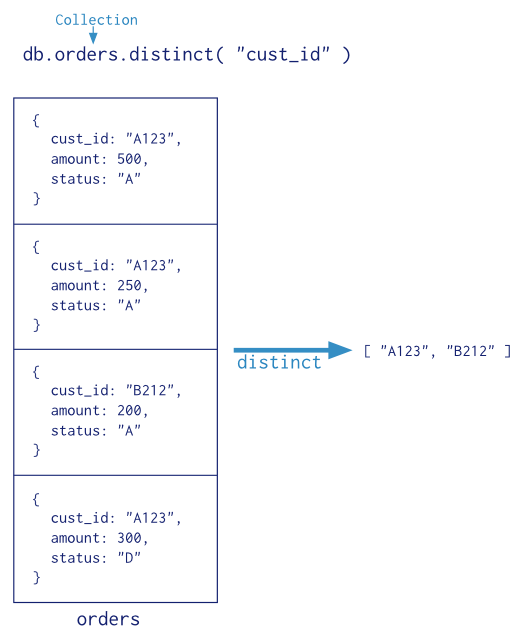
\includegraphics[width=0.5\linewidth]{distinct.png}
%\end{figure}
{\color{blue}\url{http://aurelia.io/get-started.html}}
\end{columns}
\end{frame}
%------------------------------------------------
\begin{frame}
\frametitle{Donde aprender}
\begin{columns}[c] % The "c" option specifies centered vertical alignment while the "t" option is used for top vertical alignment
\column{.45\textwidth} % Left column and width
\begin{enumerate}
\item Pagina web oficial
\item \textbf{pluralsight}
\item[•]
\end{enumerate}

\column{.5\textwidth} % Right column and width
%\begin{figure}
%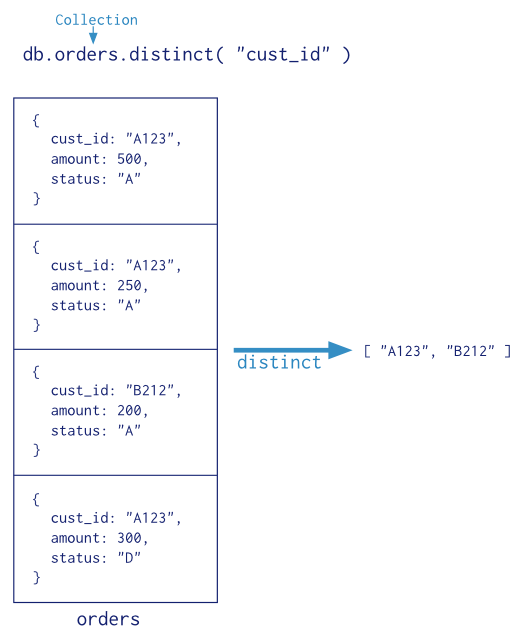
\includegraphics[width=0.5\linewidth]{distinct.png}
%\end{figure}
{\color{blue}\url{http://www.pluralsight.com/courses/building-applications-aurelia}}
\end{columns}
\end{frame}
%------------------------------------------------
\begin{frame}
\frametitle{Donde aprender}
\begin{columns}[c] % The "c" option specifies centered vertical alignment while the "t" option is used for top vertical alignment
\column{.45\textwidth} % Left column and width
\begin{enumerate}
\item Pagina web oficial
\item pluralsight
\item \textbf{youtube}
\end{enumerate}

\column{.5\textwidth} % Right column and width
%\begin{figure}
%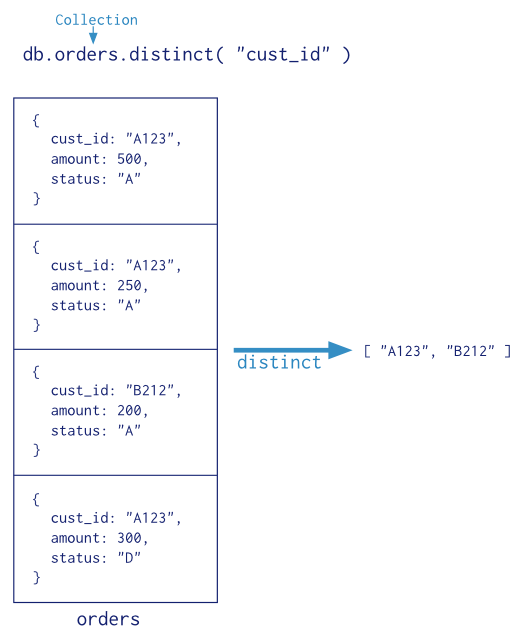
\includegraphics[width=0.5\linewidth]{distinct.png}
%\end{figure}
{\color{blue}\url{https://www.youtube.com/results?search_query=aurelia+js}}
\end{columns}
\end{frame}
%------------------------------------------------
\begin{frame}
\frametitle{Preguntas}
%\begin{figure}
%
\includegraphics[width=0.4\linewidth]{preguntas.png}
%\end{figure}
\end{frame}
%------------------------------------------------
\begin{frame}
\frametitle{Empecemos...}
\begin{figure}
%
\includegraphics[width=0.4\linewidth]{happy.png}
\end{figure}
\end{frame}
%------------------------------------------------
\begin{frame}
\Huge{\centerline{Gracias !!! =)}}
\end{frame}

%----------------------------------------------------------------------------------------

\end{document}
